\chapter{Моделирование оптической системы}

В качестве источника излучения был выбран ИК лазерный диод FPL1055T с длиной волны излучения 1550 нм, мощностью излучения в импульсном режиме 300 мВт, поперечной расходимостью 28${}^\circ$ и боковой расходимостью 15${}^\circ$~\cite{LDThorlabs}. Выбранный фотодиод \--- FDGA05 с пиковой длиной волны 1550 нм (регистрируемый диапазон длин волн 800\--1700 нм), отзывчивостью 0.95 А/Вт, площадью активной области 0.196 мм${}^2$ и материалом сенсора InGaAs~\cite{PDThorlabs}.

Для моделирования оптической системы использовался пакет Zemax OpticStudio 21.1.2. Рассмотрим задание параметров компонентов системы (рисунки~\ref{fig:no_lens_zemax_1}):

\begin{figure}[!h]
    \centering
    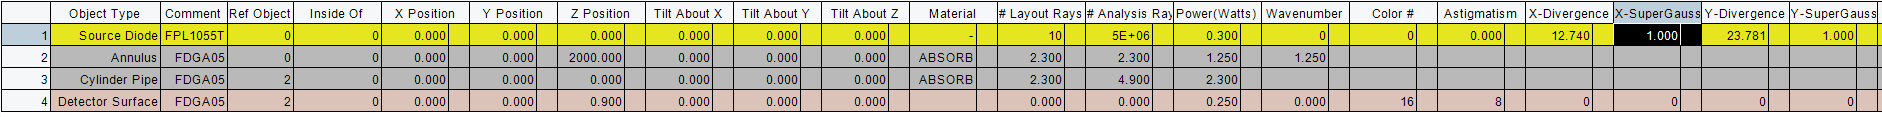
\includegraphics[width=\textwidth]{inc/img/no_lens_1.png}
    \caption{Задание параметров оптической системы в Zemax}
    \label{fig:no_lens_zemax_1}
\end{figure}

Первые 11 колонок (до колонки <<\# Layout Rays>>) универсальны для всех объектов в Zemax: тип объекта, комментарий, референтный объект, нахождение внутри другого объекта, X, Y и Z координаты, наклон вокруг осей X, Y и Z, материал объекта (где применимо). Далее идут специфические для объекта параметры:

Для диода: количество лучей для рендеринга и для расчётов (выбираются произвольно), мощность источника (выбрана в соответствии с~\cite{LDThorlabs}), номер длины волны (задаётся список используемых длин волн, задана только одна \--- 1550 нм, поэтому в ячейке стоит ноль \--- выбор любой длины волны из списка), цвет лучей на рендере, астигматизм (расстояние, на которое смещено распределение излучения в плоскости XZ), расходимость $\alpha_x$ для направления OX, супер-гауссов коэффициент $G_x$ в направлении OX, расходимость $\alpha_y$ и супер-гауссов коэффициент $G_y$ для направления OY. 

Супер-гауссов коэффициент показывает отличие профиля интенсивности данного пучка от профиля интенсивности Гауссова пучка \--- чем он больше, тем ближе профиль интенсивности излучения к прямоугольному профилю~\cite{Paschotta2008}. Для обоих направлений был выбран супер-гауссов коэффициент $G_{x,y} = 1$ (Гауссово распределение интенсивности). Следуя документации Zemax, можно рассчитать $\alpha_{x,y}$ следующим образом: 

\begin{equation*}
    \alpha_{x, y}=\frac{\theta_{\mathrm{fwhm}}}{\sqrt{2 \ln (2)}},
\end{equation*}

где $\theta_{\mathrm{fwhm}}$ \--- угол расходимости из~\cite{LDThorlabs}.

Два следующих объекта формируют корпус фотодиода: круг с отверстием и трубка. Для круга с отверстием задаются радиусы отверстия и самого круга по большой и малой полуосям. Их значения соответствуют размерам реального лазерного диода~\cite{PDThorlabs}. Его положение задаётся относительно лазерного диода.Для трубки задаются радиусы начала и конца, длина. Радиусы равны и взяты из документации к фотодиоду, длина взята произвольной, положение задаётся относительно круга с отверстием.

Для фотодиода заданы размеры апертуры (взяты из документации), количество угловых и радиальных зон оставлены по умолчанию и необходимы для расчётов в симуляции. Положение фотодиода задаётся относительно круга с отверстием и соответствует положению фотодиода в корпусе.

Для анализа системы зададим 5$\cdot \text{10}^6$ лучей, проведём трассировку лучей и получим оптическую мощность, полученную на фотодиоде. Анализ будем производить для различных расстояний между лазерным диодом и фотоприёмником. Результаты всех симуляций приведены в приложении~\ref{ch:simulation_results} в таблице~\ref{tab:distance_simulation}. Построим график зависимости оптической мощности от расстояния (рисунок~\ref{fig:distance_plot}).

\begin{figure}[h]
    \centering
    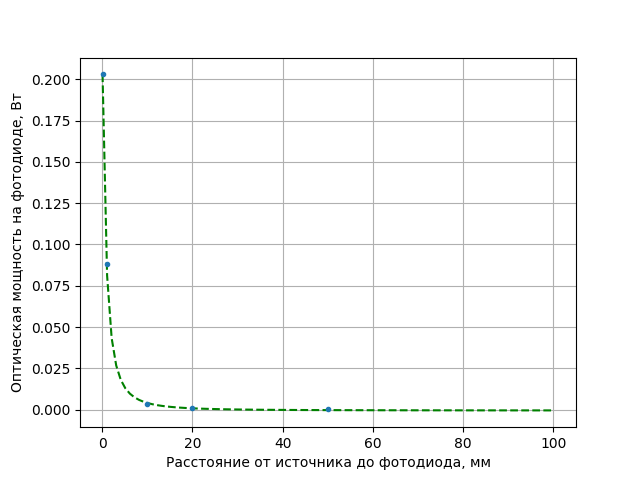
\includegraphics[width=.6\textwidth]{inc/img/distance.png}
    \caption{Зависимость оптической мощности на фотодиоде от расстояния между лазерным диодом и фотодиодом: результаты симуляции показаны синими точками, аппроксимирующая функция показана зелёной пунктирной линией}
    \label{fig:distance_plot}
\end{figure}

Эту зависимость можно аппроксимировать функцией $f(x) = \frac{1}{R^2}$, так как зависимость оптической мощности от расстояния подчиняется закону обратных квадратов. Лучшим образом для этого подходит функция $f(x) = \frac{0.615}{(x+1.639)^2} - 2.049\cdot10^{-4}$ (показана на графике пунктирной зелёной линией, результаты симуляции показаны синими точками).

Аналогично исследуем зависимость оптической мощности от угла расходимости источника при расстоянии между источником и приёмником 100 мм. Выберем одинаковые углы расходимости по обеим осям, так как приёмник симметричен. Результаты симуляции приведены в приложении~\ref{ch:simulation_results} в таблице~\ref{tab:divergence_simulation}. График результатов приведён на рисунке~\ref{fig:divergence_plot}.

\begin{figure}[h]
    \centering
    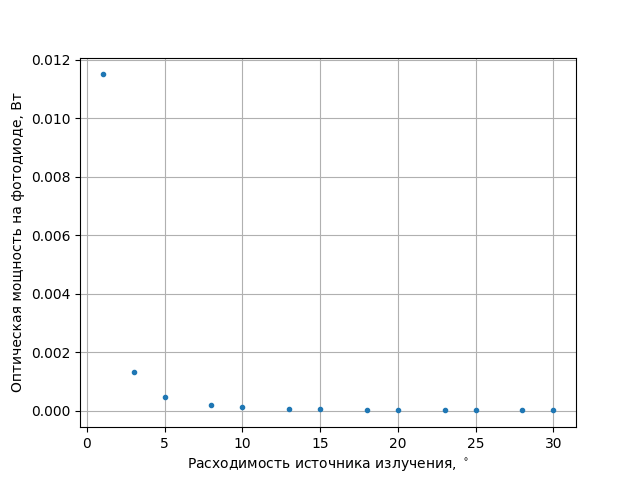
\includegraphics[width=.6\textwidth]{inc/img/divergence.png}
    \caption{Зависимость оптической мощности на фотодиоде от угла расходимости излучения лазерного диода: результаты симуляции показаны синими точками}
    \label{fig:divergence_plot}
\end{figure}

Далее добавим в систему собирающую сферическую линзу, конфигурация системы приведена на рисунке~\ref{fig:with_lens_zemax}. 

\begin{figure}[!h]
    \centering
    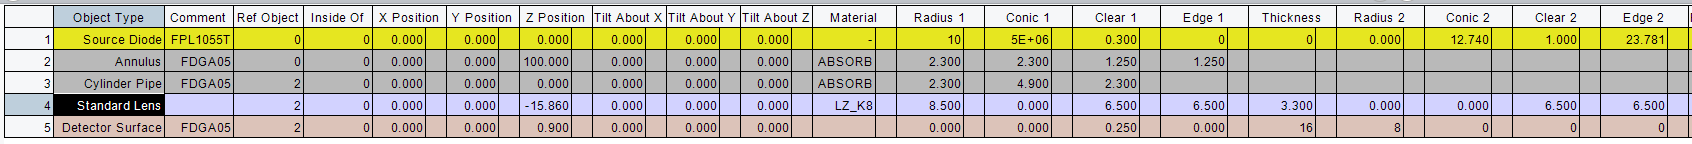
\includegraphics[width=\textwidth]{inc/img/with_lens.png}
    \caption{Задание параметров оптической системы с линзой в Zemax}
    \label{fig:with_lens_zemax}
\end{figure}

Рассмотрим параметры линзы: зададим положение линзы относительно круга с отверстием, аналогично положению фотодиода. Материал линзы \--- оптическое стекло К8 с показателем преломления $n = 1.507$ на длине волны $\lambda = 1550$ нм. Линза плоско-выпуклая с радиусом кривизны поверхности $R = 8.5$ мм, толщиной линзы $d = 3.3$ мм. Очевидно, что оптическая сила этой линзы (по формуле \eqref{eq:focal_length}) $f = 16.76$ мм. 

\begin{equation}
    \frac{1}{f} = \frac{n-1}{R}
    \label{eq:focal_length}
\end{equation}

Тогда для лучшей фокусировки лучей необходимо поместить фотодиод в фокус линзы, то есть необходимо поместить линзу на расстоянии $15.86$ мм от корпуса фотодиода (фотодиод находится на расстоянии $0.9$ мм от поверхности корпуса) \--- рисунок~\ref{fig:with_lens_zemax}. Аналогично двум предыдущим случаям, будем менять расположение линзы относительно фотодиода и наблюдать за изменением оптической мощности на приёмнике. Все результаты симуляции приведены в приложении~\ref{ch:simulation_results} в таблице~\ref{tab:lens_simulation}. График результатов приведен на рисунке~\ref{fig:lens_plot}.

\begin{figure}[h]
    \centering
    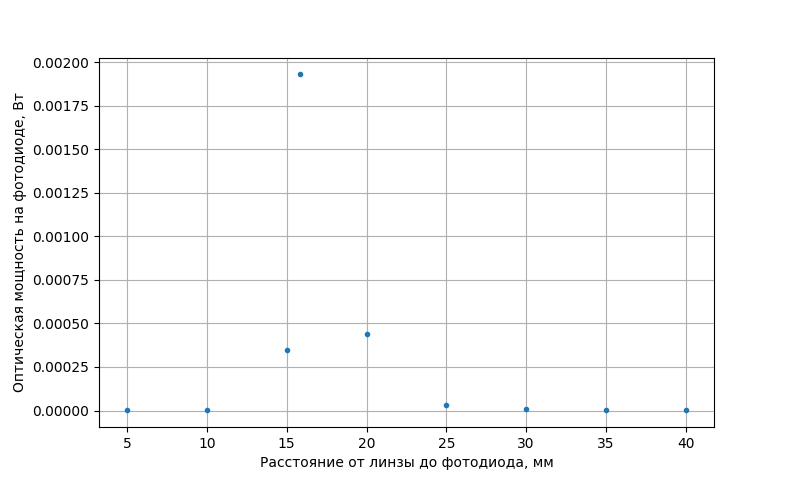
\includegraphics[width=.6\textwidth]{inc/img/lens.png}
    \caption{Зависимость оптической мощности на фотодиоде от расстояния между собирающей линзой и фотодиодом: результаты симуляции показаны синими точками}
    \label{fig:lens_plot}
\end{figure}

По графику видно, что действительно наибольшая оптическая мощность на фотодиоде наблюдается при нахождении фотодиода в фокусе линзы. 

По результатам изменения параметров видно, что самая высокая оптическая мощность достигается при наименьшем расстоянии между фотодиодом и лазерным диодом, наименьшем угле расходимости излучения лазерного диода или при установке собирающей линзы на расстоянии от фотодиода, равном фокусному. Однако даже в наилучших случаях оптическая мощность значительно меньше, чем мощность излучения источника ($0.203$ Вт, $0.0115$ Вт и $0.00193$ Вт соответственно, против $0.3$ Вт источника). Очевидно, что необходима дополнительная оптическая система для коллимации лучей источника и для фокусировки лучей у приёмника для уменьшения оптических потерь системы и для создания системы, в которой возможно передавать информацию.